\cotefile{154}
\scanpage{77}
\deleted{\unsure{antipodique d'une}}

opposée d'une arête orientée $(D,\unsure{o|a})$ :
l'arête $(D',\unsure{o'|a'})$, où $D'$ est déduite de
$D$ par balayage via $\unsure{a'=\operatorname{antip}(a)}$,
et $\unsure{o'|a'}$ \deleted{\unsure{déduite de}} \inserted{\unsure{antipodale de celle}} $=$ par \uline{transport}
parallèle, i.e. ``opposée à $\unsure{o|a}$''.

Origine de $(D,\unsure{o|a})$ est $D$

2) Structure polygonale sur l'\unsure{ens.} des arêtes
orientées issues de $D$ : évidente

3) Transport d'orientations : \uuline{\unsure{opposé}}
du transport parallèle des orientations
des \unsure{f. p.}

Hélas on ne trouve pas les bons
circuits superréguliers --- \unsure{ça ne va pas}
\unsure{bien sûr}, si alléchant que celà
paraisse ! Si cependant on modifie
3), en prenant comme sens de transport
pour les orientations le transport parallèle,
on trouve les bons circuits \uline{superréguliers}
(mais pas d'application naturelle $\unsure{\mathcal X}\to X$ !).

Il y a une autre (au moins !) possibilité
de construction encore, c'est de \unsure{recoller} $a$ à $\unsure{b'}$,
$b$ à $a'$, ainsi

\figure{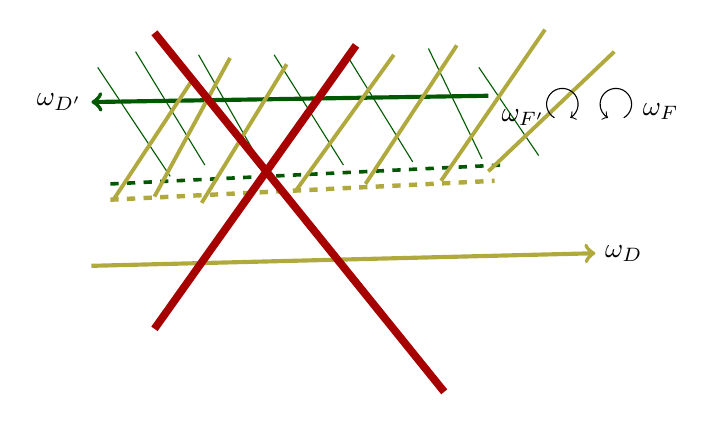
\begin{tikzpicture}[x=0.8cm,y=0.8cm]
\draw[green!35!black,line width=1.5pt,<-] (0,3.3)--(6.3,3.4);
\node[left] at (0,3.3) {$\omega_{D'}$};
\draw[yellow!65!black,line width=1.5pt,->] (0,0.7)--(8,0.9);
\node[right] at (8,0.9) {$\omega_D$};
\draw[green!35!black,line width=1.3pt,dashed] (0.3,2)--(6.5,2.3);
\draw[yellow!65!black,line width=1.6pt,dashed] (0.3,1.75)--(6.4,2.05);
\draw[green!35!black] (0.1,3.85)--(1.25,2.12);
\draw[green!35!black] (0.7,4.1)--(1.8,2.3);
\draw[green!35!black] (1.7,4.05)--(2.7,2.3);
\draw[green!35!black] (2.9,4.05)--(4,2.3);
\draw[green!35!black] (4.05,4.05)--(5.1,2.35);
\draw[green!35!black] (5.35,4.15)--(6.2,2.4);
\draw[green!35!black] (6.15,3.85)--(7.1,2.45);
\draw[yellow!65!black,line width=1.4pt] (0.35,1.75)--(1.6,3.65);
\draw[yellow!65!black,line width=1.4pt] (1,1.8)--(2.2,4);
\draw[yellow!65!black,line width=1.4pt] (1.75,1.7)--(3.1,3.9);
\draw[yellow!65!black,line width=1.4pt] (3.25,1.9)--(4.8,4.05);
\draw[yellow!65!black,line width=1.4pt] (4.35,2)--(5.8,4.2);
\draw[yellow!65!black,line width=1.4pt] (5.55,2.05)--(7.2,4.45);
\draw[yellow!65!black,line width=1.4pt] (6.3,2.2)--(8.3,4.1);
\draw[->] (7.35,3.05) arc[start angle=240,end angle=-60,radius=.25];
\node[left] at (7.35,3.05) {$\omega_{F'}$};
\draw[->] (8.45,3.05) arc[start angle=-60,end angle=240,radius=.25];
\node[right] at (8.6,3.15) {$\omega_F$};
\draw[red!65!black,line width=2.8pt] (1,4.4)--(5.6,-1.3);
\draw[red!65!black,line width=2.8pt] (1,-.3)--(4.2,4.2);
\end{tikzpicture}}

en utilisant pour le recollement le
transport parallèle, de façon donc
à avoir tjrs $\unsure{\mathcal X}\to X$, mais
cette fois pas une immersion,
mais \deleted{des} \unsure{applications|application} pliant
le long des arêtes de $K$.

La description combinatoire
est analogue à celle qui
précède, la seule modification
est dans 1) (description de
l'opposée d'une arête, \unsure{maint.} \inserted{\unsure{pour}}
l'opposée $(D',\unsure{o'|a'})$ de $(D,\unsure{o|a})$, $\unsure{o'|a'}$ est
déduite de $\unsure{o|a}$ par transport
parallèle. Pour $\unsure{2)\ \text{et}\ 3)}$, \unsure{ne rien changer}
\margin{\unsure{76}}
